% DATE OF START                                             20/11/2017
% DATE OF SUBMISSION                                          /  /2018
% DATE OF THE FIRST REFEREE REPORT ARRIVED                    /  /2018
% DATE OF RESUBMITTING THE REVISED MANUSCRIPT                 /  /2018
% DATE OF RECEIVING THE EDITORIAL DECISION                    /  /2018
% DATE OF ACCEPTANCE                                          /  /2018
%% -------------------------------------------------------------------
\documentclass[prb, twocolumn, final]{revtex4-1}
\usepackage{braket}
\usepackage{amsmath}
\usepackage{graphicx}
\usepackage{mathtools}
\usepackage{amsmath, amsfonts, amssymb, amsbsy, amsthm}


\theoremstyle{plain}
\newtheorem{theorem}{Theorem}
\newtheorem*{theorem*}{Theorem}
\newtheorem{definition}[]{Definition}
\newtheorem{lemma}[]{Lemma}
\renewcommand\thelemma{\unskip}
\renewcommand\thedefinition{\unskip}
\renewcommand{\qedsymbol}{$\blacksquare$}

% ------------------------------------------------------------------------------
% Personal definitions
% ------------------------------------------------------------------------------
% Redefining the \abs and \norm so that they automatically change their size
\DeclarePairedDelimiter\abs{\lvert}{\rvert}%
\DeclarePairedDelimiter\norm{\lVert}{\rVert}%

% Swap the definition of \abs* and \norm*, so that \abs and \norm resizes the
% size of the brackets, and the starred version does not.
\makeatletter
    \let\oldabs\abs
    \def\abs{\@ifstar{\oldabs}{\oldabs*}}
%
    \let\oldnorm\norm
    \def\norm{\@ifstar{\oldnorm}{\oldnorm*}}
\makeatother


% ------------------------------------------------------------------------------
% DOCUMENT BEGINS
% ------------------------------------------------------------------------------
\begin{document}

% ------------------------------------------------------------------------------
% TITLE PAGE
% ------------------------------------------------------------------------------
\title{Quantum recurrence}
\author{Nik Mitchell}
\author{Daniel Schumayer}
\author{David A. W. Hutchinson}
\affiliation{Department of Physics, University of Otago, Dunedin, New Zealand}
\email{daniel.schumayer@otago.ac.nz}
\date{\today}

% ------------------------------------------------------------------------------
% ABSTRACT
% ------------------------------------------------------------------------------
\begin{abstract}
    Systems of ultra-cold gases in light-induced periodic potentials, often
    called optical lattices, are of great experimental and theoretical interest,
    and have been since the first experimental realisation of Bose-Einstein
    condensation in 1995. This is largely due to the parallels between the
    behaviour of bosons on optical lattices and condensed matter systems, where
    electrons can be modelled as moving on a lattice generated by the periodic
    array of atom cores. This project investigates the time evolution of a
    system of bosons prepared in a far-from-equilibrium state on a
    one-dimensional or two-dimensional optical lattice. The key question of
    interest is whether the system relaxes to some sort of equilibrium state or
    if it exhibits exact and regular revival to the initial state.
\end{abstract}

\pacs{}
% Resolution of these PACS codes:

\maketitle


% ------------------------------------------------------------------------------
% INTRODUCTION
% ------------------------------------------------------------------------------

\section{Introduction}

\section*{Introduction}
The question of how, and under what conditions, closed quantum systems approach
thermal equilibrium is an old question that forms the basis of a large and
active field of research. Thermalisation is well understood in the context
of classical mechanics, where it emerges from the chaotic
dynamics of sufficiently unconstrained systems. However, the time evolution of
quantum systems is strictly linear, and hence they do not exhibit chaotic
dynamics. Nonetheless, there are a number of closed quantum systems in which
thermalisation is observed, in the sense that the systems relax to states in
which the values of macroscopic quantities are stationary, universal with
respect to widely differing initial conditions, and predictable using
statistical mechanics \cite{Rigol2008}.

This project investigates the time evolution of a variety of different systems
composed of non-interacting and interacting bosons on one-dimensional and
two-dimensional optical lattices that are prepared in far-from-equilibrium
states. These systems are investigated analytically where possible, and with
numerical methods for larger and more complicated systems where an analytic
approach is not tractable.

We focus primarily on gaining a strong
understanding of smaller systems of few lattice sites and bosons, as these
can be solved exactly.
%From here, we look at some larger systems with a more
% approximate method that revolves around using an adaptive Runge-Kutta-Feldberg
% method to evolve the system wavefunction according to the Gross-Pitaevskii
% equation. We then look for similarities in the results of the simulations run
% according to each method to see what how much of the behaviour of small,
% exactly solved systems is preserved is we move to large, numerically approximated
% systems. By doing so, we aim to pave the way for a systematic study of the role
% of integrability in relaxation and thermalisation of far-from-equilibrium
% quantum systems.
\newpage


\section{Experiments with optical lattices}

This project considers the thermalisation behaviour of systems of bosons on
optical lattices. One of the main factors that make these systems interesting
to work with are the deep similarities between the Hamiltonians of systems that
can be generated using bosons on an optical lattices and those of electrons
moving on a lattice potential produced by a periodic array of atom cores. We can
simulate these condensed matter systems with ultracold atoms by using optical
lattices to generate the periodic potential.

An optical lattice is produced by
overlapping multiple laser beams and making use of the interference pattern.
The alternating bright and dark areas of the interference pattern act as a
periodic potential on the atoms through the optical dipole force
\cite{Bloch2012}. By superimposing different combinations of laser beams at
particular frequencies and amplitudes, any lattice geometry that can be
constructed via Fourier synthesis can, in principle, be produced
\cite{Bloch2012}. This fine degree of control over the lattice parameters, in
conjunction with the ability to tune the strength of interparticle interactions
by manipulating Feshbach resonances \cite{Chin2010}, makes ultracold bosons on
optical lattices an excellent arena in which to explore various model
Hamiltonians for condensed matter systems and quantum optics.


%There are further advantages which can make conducting experiments with
%ultracold bosons on optical lattices more attractive than working with solids
%directly. One is that there are always impurities present in the solids we find
%in nature. These impurities can have significant impacts on the properties of
%the solid which cannot necessarily be accounted for by a perturbative approach
%which assumes these effects to be small. For large-enough detunings from an atomic
%transition frequency, optical lattices can be considered to be purely
%conservative and defect-free potentials \cite{Bloch2012}, so when dealing with
%bosons on optical lattices this problem of impurities does not arise.

%Another benefit of working with bosons on optical lattices is that we can easily
%control the state of each of the particles on the lattice. Furthermore, the
%potential can be altered or switched off entirely during the experiment, which
%is a feature that is not available in any solid state experiment
%\cite{Morsch2006}.


As we are dealing with large numbers of indistinguishable bosons, we will
exclusively use the second quantised representation, which is much more succint
as it makes no reference to unique identities of individual particles. For a
discussion of the mathematics of second quantisation, see \ref{Altland2010}.

In this formalism, the Hamiltonian that describes our system is

 have analogues in condensed matter systems. The
individual bosons will have kinetic energy, and the potential created by the
lattice also contributes to how the system evolves in time, so it must feature
in the Hamiltonian. The bosons may be interacting, and there may also be an
external potential imposed that can vary in strength from site to site.

With regards to the interparticle interactions, we consider repulsive scattering
interactions. We will consider systems that are dilute, in the sense that the
average spacing between bosons is much greater than the effective range of the
interparticle interactions. This makes it reasonable to consider only
two-particle scattering events and neglect the rare higher order collisions,
provided we keep the strength of the interparticle interactions small. Even when
reduced to its two-body form, $U(x,x')$, the form of the interatomic scattering
potential has short range terms that can be difficult to deal with. We can
replace this object with a mathematically more convenient effective potential,
corresponding to contact interaction, with the same scattering cross-section at
low energy. Because the ultracold bosons have such low energy, $s$-wave
scattering dominates, and the interparticle interaction potential can be
expressed simply in terms of the $s$-wave scattering length, $a_{s}$, as
\begin{equation}
    U_{\text{eff}}
    =
    \frac{2 \pi\hbar^{2} a_{s}}{m}
    \sum_{i,j}{\delta(x_{i} - x_{j})}.
\end{equation}
For simplicity, we will introduce the notation $U_{0} = \frac{4 \pi \hbar^{2}
a_{s}}{m}$. Having made these simplifications, we can construct a first
quantised Hamiltonian for a one-dimensional system of interacting bosons on an
optical lattice, in the presence of an external potential $V_{\text{ext}}$
\begin{equation}
    \label{eq:HamiltonianCoordinateRepresentation}
    \hat{h}
    =
    \sum_{i}{-\frac{\hbar^{2}}{2m}  \partial_{x_{i}}^{2}} +
    \sum_{i}{V_{\text{lattice}}(R_{i})} +
    V_{\text{ext}}(x) +
    \frac{U_{0}}{2} \sum_{i,j}{\delta(x_{i} - x_{j})}.
\end{equation}
Similar Hamiltonians are frequently used to describe systems of electrons on
atomic lattices. To promote conciseness, we introduce the abbreviations
\begin{equation*}
    \hat{h}_{1}
    =
    \sum_{i}{-\frac{\hbar^{2}}{2m} \partial_{x_{i}}^{2}} +
    \sum_{i}{V_{\text{lattice}}(R_{i})},
    \quad
    \hat{h}_{\text{ext}}
    =
    V_{\text{ext}}(x),
    \quad
    \hat{h}_{\text{int}}
    =
    \frac{U_{0}}{2} \sum_{i,j}\delta{(x_{i}-x_{j})}
\end{equation*}
so that $\hat{h}=\hat{h}_1+\hat{h}_{\text{ext}}+\hat{h}_{\text{int}}$.


\section{The Bose-Hubbard model}

The Hamiltonian for a weakly interacting BEC in a one-dimensional optical
lattice and subject to harmonic trapping potential is given by the sum of
$\hat{H}_{1}$, $\hat{H}_{\text{ext}}$ and $\hat{H}_{\text{int}}$:
\begin{equation}
    \hat{H}_{\text{1D}}
    =
    J \sum_{i}{(\hat{a}^\dagger_{i}\hat{a}_{i+1} + \text{h.c.})} +
    \frac{U_{0}}{2}
    \sum_{i}%
        {\hat{a}_{i}^{\dagger} \hat{a}_{i}^{\dagger} \hat{a}_{i} \hat{a}_{i}} +
    \sum_{i}%
        {\epsilon_{i} \hat{a}_{j}^{\dagger} \hat{a}_{j}},
\end{equation}
and is known as the Bose-Hubbard Hamiltonian. The $\epsilon_{i}$'s refer to
on-site energies at each lattice site due to the harmonic trap, and the middle
term gives an interaction energy when there is more than one particle on a
particular site. This project will look at scenarios where there is no external
harmonic potential which produces different on-site energies for different sites
(the uniform lattice potential remains, so $J$ is still defined as before). In
the absence of this external potential, the Hamiltonian in one dimension reduces
to
\begin{equation*}
    \hat{H}_{1D}
    =
    J \sum_{i}{(\hat{a}^\dagger_{i}\hat{a}_{i+1} + \text{h.c.})} +
    \frac{U_{0}}{2}
    \sum_{i}{\hat{a}^\dagger_{i} \hat{a}^\dagger_{i} \hat{a}_{i}\hat{a}_{i}}.
\end{equation*}

This project aims to explore the dynamics of both this one-dimensional system
and the two-dimensional version where we couple multiple chains of lattice
sites together. The system Hamiltonian in two dimensions is
\begin{equation}
    \hat{H}_{2D}
    =
    \left (
        J \sum_{i,j}{\hat{a}^{\dagger}_{i,j+1} \hat{a}_{i,j}} +
        J'\sum_{i,j}{\hat{a}^{\dagger}_{i,j} \hat{a}_{i+1,j}}
    \right) +
    \text{\text{h.c.}} +
    \frac{U_{0}}{2}
    \sum_{i}{\hat{a}^{\dagger}_{i}\hat{a}^{\dagger}_{i} \hat{a}_{i}\hat{a}_{i}},
\end{equation}
where the $i$ index denotes which chain is being referred to and the $j$ index
denotes how far along the chain a site is. $J'$ is another hopping parameter,
in this case characterising the hopping between sites on different chains.
\begin{figure}[H]
    \begin{center}
        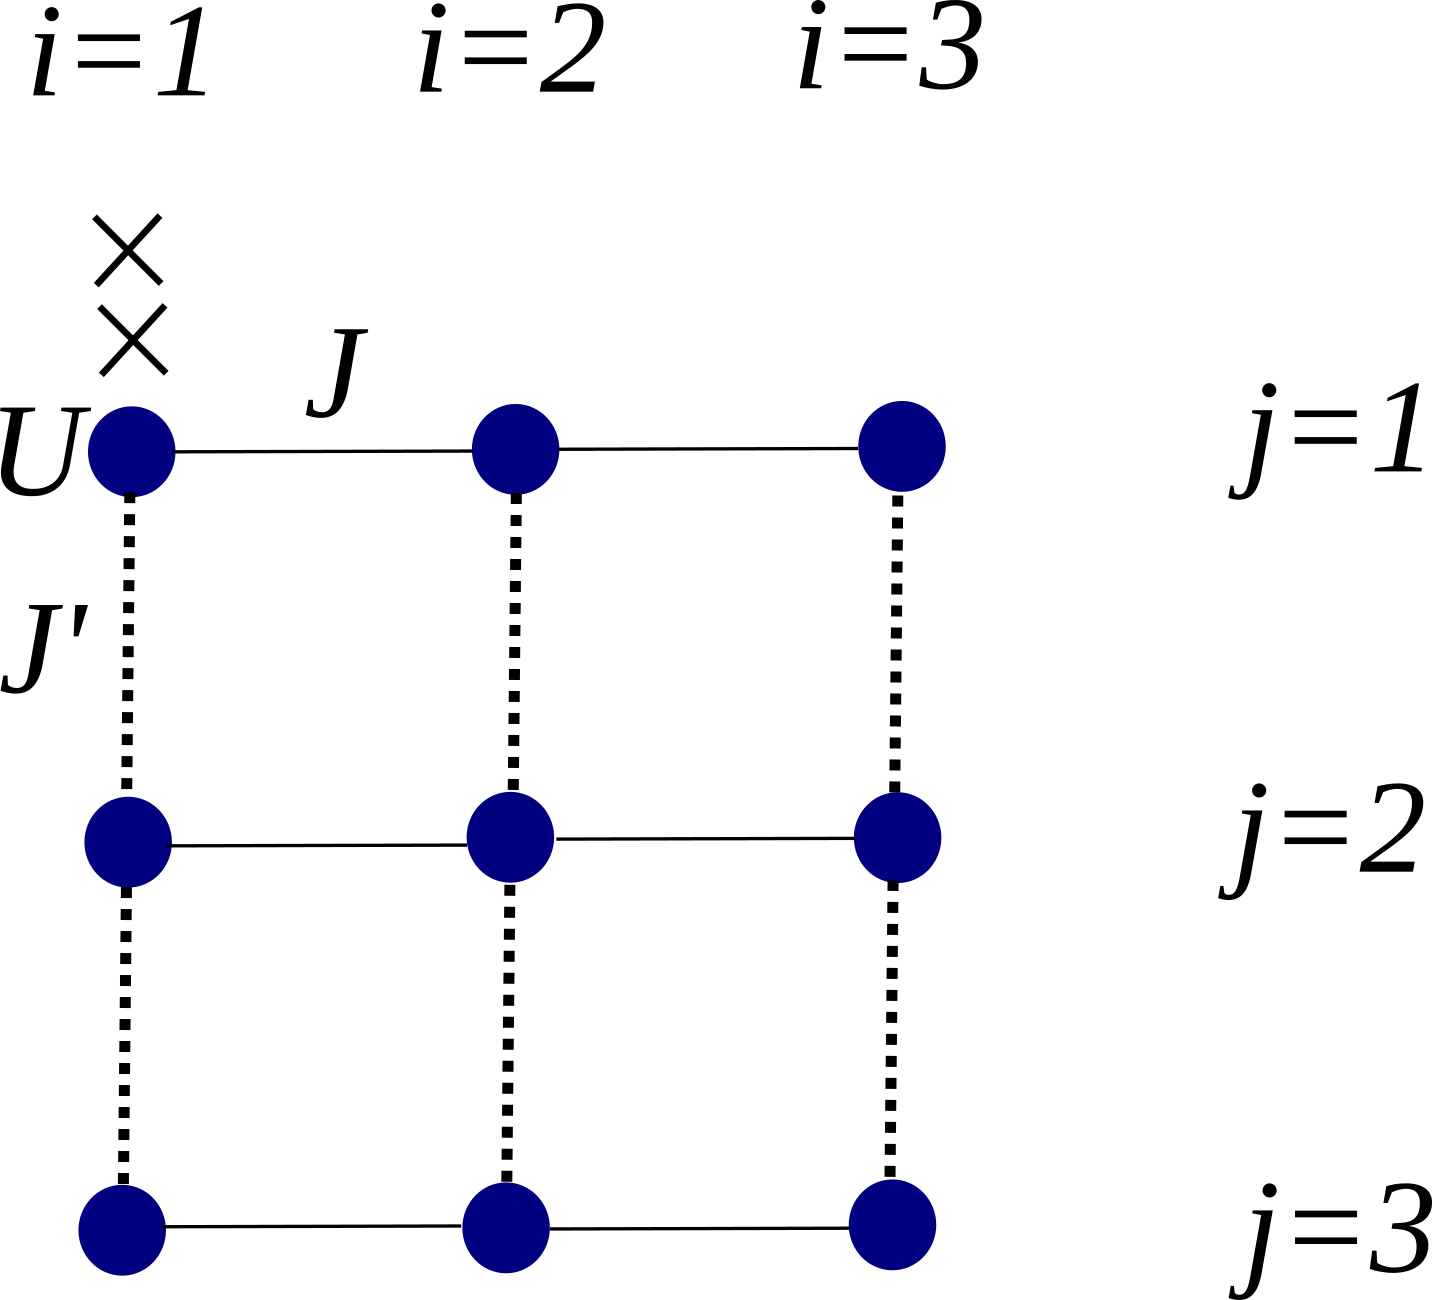
\includegraphics[width=8cm]{./Figures/lattice_pic.png}
    \end{center}
    \caption{The blue circles here represent lattice sites and the crosses
             denote individual bosons. Hopping between any two neighbouring
             sites on the same chain is characterised by $J$, whereas hopping
             between chains is characterised by $J'$. A three by three lattice
             is shown here, but the system can be extended to arbitrary size.
            }
\end{figure}
We are interested in the time evolution of these systems as it relates to their
thermal behaviour.


\section{Thermalisation}

Thermalisation refers to a relaxation of a system to states where the values
of macroscopic quantities are stationary, universal with respect to widely
differing initial conditions, and predictable using statistical mechanics
\cite{Rigol2008}. We observe thermalisation in a wide variety of classical
systems, and there are strong theoretical reasons for anticipating this
thermalisation. However, many of these reasons don't apply when considering
quantum systems, since the time evolution for quantum systems is linear.

\newpage
\section{System size and analyticity}

Whilst the main focus of this project is on smaller lattices with few particles,
it is of interest to investigate larger system sizes (necessarily by approximate
methods) to see how much of the qualitative behaviour of the small systems is
preserved in the larger ones.

\subsection{Dimensionality of many-body systems}

We can decompose any time evolved state $\ket{\psi(t)}$ of our system in terms
of its state at $t=0$, $\ket{\psi(0)}$, and the energy eigenvectors $\ket{E_n}$
(see section \ref{revival} for details):
\begin{equation}
    \label{eq:SmallSystems_PsiTimeEvolution}
    \ket{\psi(t)} = \sum_{j}{e^{i E_{j}t} \ket{E_{j}} \braket{E_{j}|\psi(0)}}.
\end{equation}
Calculating $\ket{\psi(t)}$ from the above formula requires that we diagonalise
the Hamiltonian and find its energy eigenvectors and eigenvalues. This is easy
for small systems, in particular those that have only a single particle on them.
This method has the significant advantage of being ``analytic'', at least up to
the precision of the values stored for the eigenvalues and eigenvectors.
However, as the number of lattice sites and
particles in the system increases, the time required to apply this method
increases dramatically. This is because the dimensionality $\mathcal{D}$ of the
system grows according to
\begin{equation}
    \label{dimensionality_exact}
    \mathcal{D} = \frac{(N + P - 1)!}{P! (N-1)!},
\end{equation}
where $N$ is the number of lattice sites and $P$ is the number of particles on
the lattice. Unsurprisingly, this is the same as the number of possible pure
number states (since these form an orthonormal basis), and so the formula
deduced is just the formula for the number of ways to arrange $P$ objects into
$N$ containers that is familiar from elementary statistical mechanics.
The Hamiltonian can be represented in the basis of energy eigenvalues as a
$\mathcal{D} \times \mathcal{D}$ square matrix. However diagonalising this
matrix, determining its energy eigenvalues and then evolving the system
according to equation \eqref{eq:SmallSystems_PsiTimeEvolution} quickly becomes
impractical for systems with large numbers of particles and lattice sites.


\section{Results}

\section{Revival \label{revival}}

In a subset of the integrable systems considered, we observed regular instances
in which the system would return to the state in which it was initially
prepared (it ``revives''). To see why we might expect to see revival in
some cases, consider the initial state of the system $\ket{\psi(0)}$, which
evolves in time according to
\begin{equation}
    \ket{\psi(t)} = e^{i \hat{H} t} \ket{\psi(0)},
\end{equation}
where --for sake of brevity and transparency-- the constant $\hbar^{-1}$ has
been incorporated into the time scale. Now noting that we can use the
completeness relation for the energy eigenstates to expand the initial state in
the energy basis one obtains
\begin{align}
\label{time_evolution}
 \ket{\psi(t)} &= e^{i\hat{H}t}\sum_j\ket{E_j}\braket{E_j|\psi(0)}  \nonumber \\
               &= \sum_je^{i\hat{H}t}\ket{E_j}\braket{E_j|\psi(0)}  \nonumber \\
               &= \sum_je^{iE_{j}t}\ket{E_j}\braket{E_j|\psi(0)}    \nonumber \\
               &= \sum_j c_{j}e^{iE_{j}t}\ket{E_j}.
\end{align}
From here it can be seen that the only time dependence appears in the complex
exponentials, each of which is $2 \pi$-periodic. If we can find some common time
$t^{\ast}$ such that $E_{j} t^{\ast} = 2 \pi k_{j}$, where $k_{j} \in\mathbb{Z}$
for all $j$, we will recover the initial state exactly, i.e.,
$\ket{\psi(t^{\ast})} = \ket{\psi(0)}$. The next section describes the
conditions necessary for the existence of the revival time.


\subsection{Exact revival}

We observe an exact and regular revival in precisely the cases in which the
eigenvalues are mutually rational, i.e., they are either all rational, or are
all rational when divided by the same irrational number.
\begin{definition}[Mutually rational set]
    We say that a set of eigenvalues are mutually rational if they are all
    rational when divided by a common real number.
\end{definition}
For example, the set of hypothetical eigenvalues $\lbrace 0, \sqrt{2}, 2
\sqrt{2}, \frac{3 \sqrt{2}}{10} \rbrace$ is mutually rational, whereas $\lbrace
0, \sqrt{2}, \sqrt{3}\rbrace$ is not. In the case of mutually rational
eigenvalues, we can write $E_{j} = \frac{p_{j}}{q_{j}}$, where $p_{j}$, $q_{j}
\in \mathbb{Z}$. The revival time is then given by
\begin{equation}
    \label{revival_time_formula}
    t^{\ast} = \frac{2 \pi Q_{\text{LCM}}}{P_{\text{HCF}}},
\end{equation}
where $Q_{\text{LCM}}$ is the lowest common multiple of $\lbrace q_{j} \rbrace$
and $P_{\text{HCF}}$ is the highest common factor of the $\lbrace p_{j} \rbrace$.

We are yet to find any systems with nonzero interparticle interaction that have
mutually rational eigenvalues. In one dimension, the only systems that we have
found that meet the criterion of mutually irrational eigenvalues are those with
fewer than 4 lattice sites. In two dimensions, the only systems that exhibit
revival have three or fewer chains and three or fewer lattice sites on each
chain (see section \ref{2Dsystems}).

To demonstrate this exact revival, consider a one-dimensional lattice with three
sites with a single boson and hopping constant $J$. The Hamiltonian for this
system is
\begin{equation}
    \hat{H}_{3\times1}
    =
    \begin{pmatrix}
         0 & -J &  0 \\
        -J &  0 & -J \\
         0 & -J &  0
    \end{pmatrix}.
\end{equation}
Diagonalising this matrix yields the eigenvalues $\lbrace -\sqrt{2}J, 0,
\sqrt{2} J \rbrace$. These are mutually rational (if we divide them all by
$\sqrt{2}J$ they are all rational). If we rescale the energies by $\sqrt{2}J$ by
absorbing that factor into the time scale, then we get eigenvalues $\{-1,0,1\}$.
We can see from the graph of the simulation below that this matches up with a
return to the initial state at times that are multiples of $2\pi$.
\begin{figure}[H]
%     \centering
%     \begin{gnuplot}[terminal=cairolatex, terminaloptions={lw 2}, scale=0.95]
%         set xlabel "$\\displaystyle \\frac{t}{\\sqrt{2}J}$"
%         set ylabel "$\\langle n_{1} \\rangle$"
%         plot "./Data/20170912T164043_evolution_n.dat" u 1:4 w l lc 1 notitle
%      \end{gnuplot}
%      \vspace*{-5mm}
     \label{fig:3by1_noninteract_revival}
     \caption{Revival for a system with 3 lattice sites and a single boson.}
\end{figure}
The reason that there appear to be several revivals that our method ``misses''
is that states with different phases in the coefficients of the eigenvectors
can also produce $\langle n_{1} \rangle = 1$, whereas the revival time that is
calculated in our method corresponds to exact revival of the initial
wave function and not $\langle n_{1} \rangle \sim \norm{\psi(t)}^{2}$.


\subsection{Approximate revival}

The range of systems for which the eigenvalues are mutually rational is a small
one. All systems which have nonzero interparticle interactions have mutually
irrational eigenvalues. One of the most interesting results so far is that
even in the one-dimensional single particle case, if there are more than
three lattice sites, the eigenvalues will be irrational. We can demonstrate this
by considering a single chain of five sites with one boson. The Hamiltonian for
this system is
\begin{equation}
    \hat{H}_{5\times1}
    =
    \begin{pmatrix}
         0 & -J &  0 &  0 &  0 \\
        -J &  0 & -J &  0 &  0 \\
         0 & -J &  0 & -J &  0 \\
         0 &  0 & -J &  0 & -J \\
         0 &  0 &  0 & -J &  0
    \end{pmatrix}.
\end{equation}
The eigenvalues of this system are $\lbrace -\sqrt{3}J, -J, 0, J, \sqrt{3}J
\rbrace$. These are clearly not mutually rational, so we cannot find an exact
revival time for this system, despite the fact that it is fully integrable
\cite{Rigol2007}.

Note that the eigenvalues of a system with $4$ lattice sites are also mutually
irrational as they are
\begin{equation*}
    \frac{J}{2}\,
    \left \lbrace
        -1 - \sqrt{5}, 1 + \sqrt{5}, 1 - \sqrt{5}, -1 + \sqrt{5}
    \right \rbrace
\end{equation*}
but those for a system of 5 lattice sites are more convenient to work with.

Running a simulation of this system of $5$ lattice sites where we start a single
boson off on the first site, we find that the probability of finding the boson
on the first site never quite reaches unity again.
\begin{figure}[H]
%     \centering
%     \begin{gnuplot}[terminal=cairolatex, terminaloptions={lw 2}, scale=0.95]
%         set xlabel "$\\displaystyle \\frac{t}{J}$"
%         set ylabel "$\\langle n_{1} \\rangle$"
%         plot "./Data/5by1_T1e4.dat" u 1:6 w l lc 1 notitle
%      \end{gnuplot}
%      \vspace*{-5mm}
     \caption{Absence of exact revival for a system with 5 lattice sites and a
              single boson.}
\end{figure}

Judging the figure above by eye, it may appear that we have exact revival, but
this is not actually the case. If we look at how long it takes for the system to
get within $\epsilon$ of its initial state (i.e. $\norm{\ket{\psi(t)} -
\ket{\psi(0)}} < \epsilon$) we get the graph below. Note that $t^{\ast}$ denotes
the time at which the system got within a particular value of $\epsilon$ of the
initial state the first time after $t=0$.
\begin{figure}[H]
    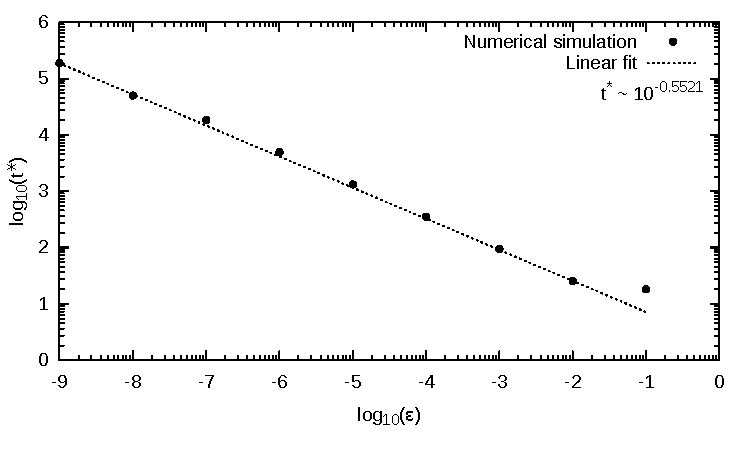
\includegraphics[width=1.0\textwidth]{./Figures/recurrence_times.pdf}
    \centering
    \label{1Drecurrencetimes}
    \caption{Recurrence times for varying values of $\epsilon$.}
\end{figure}
While we see that the system does appear to get arbitrarily close to revival,
but it can take arbitrarily long to do so. This result can be explained in terms
of the Poincar{\'e} recurrence theorem.


\subsection{The Poincar\'e Recurrence Theorem}

In 1890, Henri Poincar{\'e} proved \cite{Poincare1890, Poincare2017} the
following theorem for classical mechanics:
\begin{quote}
    Any phase-space configuration $(q, p)$ of a system enclosed in a finite
    volume will be repeated as accurately as one wishes after a finite (be it
    possibly very long) interval of time.
\end{quote}
This theorem was extended to quantum systems in 1956 by P. Bocchieri and A.
Loinger \cite{Bocchieri1957}, where they gave a slightly different form:
\begin{theorem*}[Quantum recurrence]
    Let us consider a system with discrete energy eigenvalues $E_{n}$; if
    $\Psi(t_{0})$ is its state vector in the Schr{\"o}dinger picture at the time
    $t_{0}$ and $\epsilon$ is any positive number, at least one time $t^{\ast}$
    will exist such that the norm $\norm{\Psi(t^{\ast}) - \Psi(t_{0})}$ of the
    vector $\Psi(t^{\ast}) - \Psi(t_{0})$ is smaller than $\epsilon$.
\end{theorem*}
The interested reader may refer to their paper for the proof.

\subsection{Large one-dimensional systems}

To determine the mutual rationality or mutual irrationality of the eigenvalues
for an arbitrarily large one-dimensional system with a single particle, we look
to a recent result about the eigenvalues of tridiagonal matrices proven by
W.~Yueh \cite{Yueh2006}. A tridiagonal matrix has the form
\begin{equation}
    A_{N \times N}
    =
    \begin{pmatrix}
             b &      c &     0  &      0 &  \dots & 0 \\
             a &      b &     c  &      0 &  \dots & 0 \\
             0 &      a &     b  &      c &  \dots & 0 \\
             0 &      0 &     a  &      b &  \dots & 0 \\
        \vdots & \vdots & \vdots & \vdots & \ddots & c \\
             0 &      0 &     0  &      0 &      a & b
    \end{pmatrix}.
\end{equation}
It was shown that the eigenvalues of $A_{N \times N}$ are given by
\begin{equation}
    \label{tridiagonal_eigenvalues_formula}
    \lambda_{k} = -b + 2 \sqrt{ac} \cos{\!\left( \frac{k \pi}{N+1} \right )},
\end{equation}
where $k=1$, 2,\dots, $N$. The Hamiltonian of any one-dimensional system with
$N$ sites and a single particle has exactly this form, namely
\begin{equation}
    \hat{H}_{N}
    =
    \begin{pmatrix}
         0 &     -J &     0  &      0 &  \dots &  0 \\
        -J &      0 &    -J  &      0 &  \dots &  0 \\
         0 &     -J &     0  &     -J &  \dots &  0 \\
         0 &      0 &    -J  &      0 &  \dots &  0 \\
    \vdots & \vdots & \vdots & \vdots & \ddots & -J \\
         0 &      0 &     0  &      0 &     -J &  0
    \end{pmatrix},
\end{equation}
and consequently has eigenvalues ($k=1$, 2, \dots, $N$)
\begin{equation}
    \label{1D_eigenvalues}
    E_{k} = 2 J \cos{\!\left( \frac{k \pi}{N+1} \right)}.
\end{equation}
Including multiplicities one expects $N$ eigenvalues for $\hat{H}_{N}$. The
number of $k$ values in \eqref{1D_eigenvalues} is indeed $N$. Taking into
account that $\cos{\!(\cdot)}$ is a strictly monotonically decreasing function
in $(0, \pi)$ we can conclude that the system has no degenerate energy
eigenvalues.

The set of energy eigenvalues is particularly interesting when combined with
Niven's theorem \cite{DoubleIvan}.

\begin{theorem*}[Niven's theorem]
    If $\theta$ is rational in degrees, say $\theta=2\pi r$ for some rational
    number $r$, then the only rational values of the trigonometric functions of
    $\theta$ are as follows: $\sin{\!(\theta)}$, $\cos{\!(\theta)} = 0$, $\pm
    \frac{1}{2}, \pm 1$; $\sec{\!(\theta)}$, $\csc{\!(\theta)} = \pm 1$, $\pm 2$;
    and $\tan{\!(\theta)}$, $\cot{\!(\theta)} = 0$, $\pm 1$.
\end{theorem*}
In other words, this theorem tells us that if $x$ is rational \textit{in
degrees}, then the only possible rational values of $\cos(x)$ are $0, \pm
\frac{1}{2}$ and $\pm 1$. Note in our case that $\frac{k\pi}{N+1}\neq 0, \pi$
for $k=1, 2, \dots, N$, so $\cos{\!(\frac{k\pi}{N+1})} \neq \pm 1$ and we are
left with $3$ rational options.

When we are evaluating in degrees, equation \eqref{1D_eigenvalues} becomes
\begin{equation}
    E_{k} = 2 J \cos{\!\left ( \frac{180k}{N+1} \right )}.
\end{equation}
The argument of cosine here is clearly rational since $N$ and $k$ are integers.
Hence we know that for a system with non-degenerate eigenvalues, there can be at
most three eigenvalues, $\lbrace 0, \pm \frac{J}{2} \rbrace$, that are rational.
So $\mathcal{D} \leq 3$ for a system with all eigenvalues rational (the lattice
must have at most 3 sites). We must have at least $(N-3)$ irrational eigenvalues
for any larger system size.

The spectrum of a one-dimensional system with $N$ sites and a single particle
has proven to be \eqref{1D_eigenvalues}. It is apparent that $E_{k}$ is a
strictly monotonically decreasing function as $k$ increases because $\cos(x)$ is
strictly monotonically decreasing on the interval $x\in(0,\pi)$ and $0 <
\frac{k\pi}{N+1} < \pi$ for $k=1,\dots,N$. Thus, $E_{k_{2}} < E_{k_{1}}$
whenever $k_{1} < k_{2}$. We have shown --invoking Niven's theorem-- that for
all $N>3$ the values of the cosine function are irrational. However, this result
on its own does not guarantee the violation of recurrence, as the latter notion
requires the energy eigenvalues to be {\emph{mutually}} irrational. We thus have
to prove that there is no such case when all eigenvalues are the multiples of
the same irrational number.

Below we answer the question: is there a {\emph{rational}} $\gamma$ such that
$E_{k_{1}} = \gamma E_{k_{2}}$ for $k_{1} \ne k_{2}$?

\begin{theorem*}[Mutual Rationality Recurrence Theorem]
    Consider the sequence of energy eigenvalues
    \begin{equation*}
        E_{k} = \cos{\!\left ( \frac{k \pi}{N+1} \right )}
        \qquad k=1, 2, \dots N
    \end{equation*}
    where $N >3$. There are no pair of integers, $k_{1}$ and $k_{2}$, and
    rational number $\gamma$ such the equality $E_{k_{1}} = \gamma E_{k_{2}}$ is
    satisfied.
\end{theorem*}
\begin{proof}
    First we notice that if the equality $E_{k_{1}} = \gamma E_{k_{2}}$ is
    satisfied for a particular triplet $(k_{1}, k_{2}, \gamma)$ with a rational
    $\gamma$, then swapping the indices and taking the reciprocal of $\gamma$
    also leads to a satisfactory triplet, $(k_{2}, k_{1}, \frac{1}{\gamma})$.
    Thus the rationality of $\gamma$ does not depend on whether $k_{1}$ is
    bigger than $k_{2}$ or the other way around.

    Without restricting generality we may assume that $k_{1} < k_{2}$. Therefore
    $E_{k_{1}} > E_{k_{2}}$ and consequently $\abs{\gamma} > 1$. Let us
    substitute the explicit expression of the spectrum in the equation
    \begin{align*}
        E_{k_{1}}
        &=
        \gamma E_{k_{2}}
        \\
        2 J \cos{\!\left ( \frac{k_{1} \pi}{N+1} \right )}
        &=
        2 J \cos{\!\left ( \frac{k_{2} \pi}{N+1} \right )}.
    \end{align*}
    This equation can be simplified by dividing both sides by $2J$, and using
    Euler's complex exponential expression for the trigonometric functions:
    \begin{equation*}
        \exp{\!\left ( i \,\frac{k_{1} \pi}{N+1} \right )}
        =
        \gamma \exp{\!\left ( i\,\frac{k_{2} \pi}{N+1} \right )}.
    \end{equation*}
    We have to keep in mind though that we only demand the equality of the real
    parts. Since there is no such $k$ value that $\cos{\!\bigl(\frac{k}{N+1}
\,\pi \bigr)}=
    0$, we may divide both sides of the equation above with the exponential on
    the right hand side:
    \begin{equation*}
        \exp{\!\left ( i\,\frac{k_{1}-k_{2}}{N+1} \,\pi\right )} = \gamma.
    \end{equation*}
    Raising both sides to the power of $(N+1)$ leads us to
    \begin{equation}
        \label{eq:NiksTheoremTranscendentalVsRational}
        e^{i (k_{1}-k_{2}) \pi} = \gamma^{N+1}.
    \end{equation}
    Notice that $e^{i (k_{1}-k_{2}) \pi} = (e^{i\pi})^{(k_{1}-k_{2}) } =
    (-1)^{k_{1}-k_{2}}$. Since both $k_{1}$ and $k_{2}$ are integers their
    difference is also an integer number, thus the left hand side of equation
    \eqref{eq:NiksTheoremTranscendentalVsRational} is $\pm 1$ depending on the
    parity of $(k_{1}-k_{2})$. Meanwhile the right hand side of equation
    \eqref{eq:NiksTheoremTranscendentalVsRational} is $\gamma^{N+1}$, where
    $\abs{\gamma} > 1$, therefore $\abs{\gamma^{N+1}} > 1$. Consequently this
    equation cannot have a solution triplet $(k_{1}, k_{2}, \gamma)$, where
    $k_{1}$, $k_{2}$ are integers between 1 and $N$ inclusively and $\gamma$ is
    rational.
\end{proof}

We have actually proven a much stronger statement than we needed. Here we showed
that it is not possible to chose only two eigenvalues from $E_{k}$ which are
rational multiple of each other.

Hence, we have shown that all one-dimensional non-interacting systems with more
than three lattice sites should not exhibit recurrence, which has implications
for thermalisation in these systems. To the best of our knowledge, this is a
novel result that has not previously been presented elsewhere.


\subsection{Interacting one-dimensional systems}

Adding multiple interacting particles introduces a number of interesting
features in the thermalisation properties of our system. We have found that when
weak interactions are present, thermalisation appears to occur in all
one-dimensional systems, including those that exhibited clear and regular
revival in the non-interacting case. We also note that with weak interactions the
long-term average for the expectation value of the number operators all tend
towards $\frac{P}{N}$, i.e., the particles become evenly distributed on the
lattice. With stronger interactions, however, we observe localisation, which we
will investigate in section \ref{changing_interaction_strength}.

To see why the systems that exhibited revival in the non-interacting case
thermalise once interactions are added, we consider the specific case of
two bosons on a $3\times1$ lattice. In the absence of interactions, this
is identical to a single boson on a $3\times1$ lattice, up to normalisation.
We can see from figure $8$%\ref{fig:3by1_noninteract_revival}
that we have exact revival
in this system. Once we have multiple particles with interactions in the system,
we need a larger dimensional basis to represent all of the distinct number
states, and thus we need a larger Hamiltonian. We need to pick a labelling
convention for our number states in order to define the representation of
the Hamiltonian matrix. In this project, we have chosen to label the states
in such a way that the states with the lowest index have the most particles on
one particular site of the lattice. For example ion a $3 \times 1$ system with
$2$ particles the number of number states is
\begin{equation*}
    \mathcal{D}_{3 \times 1} =
    \frac{(N + P - 1)!}{P! (N-1)!} =
    \frac{(3 + 2 - 1)!}{2! (3-1)!} = \frac{4!}{2! 2!} = 6
\end{equation*}
and the corresponding number states can be labelled as
\begin{equation*}
    \ket{200} = \ket{1},\,
    \ket{110} = \ket{2},\,
    \ket{101} = \ket{3},\,
    \ket{020} = \ket{4},\,
    \ket{011} = \ket{5},\,
    \ket{002} = \ket{6}.
\end{equation*}
Using this basis, we can represent the Hamiltonian as
\begin{equation}
    \hat{H}_{3\times1}^{\left(P=2\right)}
    =
    \begin{pmatrix}
             U & -\sqrt{2}J &          0 &   0 &          0 &          0 \\
    -\sqrt{2}J &          0 & -\sqrt{2}J &  -J &          0 &          0 \\
             0 & -\sqrt{2}J &          U &   0 & -\sqrt{2}J &          0 \\
             0 &         -J &          0 &   0 &         -J &          0 \\
             0 &          0 & -\sqrt{2}J &  -J &          0 & -\sqrt{2}J \\
             0 &          0 &          0 &   0 & -\sqrt{2}J &          U
    \end{pmatrix}.
\end{equation}
The eigenvalues of this system are
\begin{align*}
    \lambda_{1}
    &=
    U_{0}
    \\
    \lambda_{2}
    &=
    \frac{1}{2} \left(U_{0} - \sqrt{8J^2 + U_{0}^2}\right)
    \\
    \lambda_{3}
    &=
    \frac{1}{2}(U_{0} + \sqrt{8J^2 + U_{0}^2})
    \\
    \lambda_{4}
    &=
    \frac{U_{0}}{3} -
    \frac{-24 J^{2} - U_{0}^2}
         {
          3 \left (
                9 J^{2} U_{0} + U_{0}^3 + 3 \sqrt{3} \Lambda
            \right)^{\frac{1}{3}}}
    +
    \frac{1}{3}
    \left ( 9 J^{2} U_{0} + U_{0}^{3} + 3\sqrt{3} \Lambda \right )^{\frac{1}{3}}
    \\
    \lambda_{5}
    &=
    \frac{U_{0}}{3} +
    \frac{(1 + i \sqrt{3})(-24 J^{2} - U_{0}^{2})}
         {6
          \left (
              9 J^{2} U_{0} + U_{0}^{3} + 3 \sqrt{3} \Lambda
          \right )^{\frac{1}{3}}
         }
    -
    \frac{1}{6} (1 - i \sqrt{3})
    \left (
        9 J^{2} U_{0} + U_{0}^{3} +
        3 \sqrt{3} \Lambda
    \right )^{\frac{1}{3}}
    \\
    \lambda_{6}
    &=
    \frac{U_{0}}{3} +
    \frac{(1 - i\sqrt{3})(-24 J^{2} - U_{0}^{2})}
         {6
          \left (
              9 J^{2} U_{0} + U_{0}^{3} +
              3 \sqrt{3} \Lambda
          \right )^{\frac{1}{3}}
         }
    -
    \frac{1}{6} (1 + i\sqrt{3})
    \left (
        9 J^{2} U_{0} + U_{0}^{3} +
        3 \sqrt{3} \Lambda
    \right )^{\frac{1}{3}}
\end{align*}
where we introduced the temporary shorthand notation of
\begin{equation*}
    \Lambda = \sqrt{-512 J^{6} - 61 J^{4} U_{0}^{2} - 2 J^{2} U_{0}^{4}}.
\end{equation*}
Whilst we have not proven that the above eigenvalues form a mutually irrational
set, when we consider the number of square roots and third roots in the above
set of eigenvalues, we see that it at least appears very unlikely that a
particular combination of $J$ and $U_{0}$ would result in a mutually rational
set of eigenvalues.

When we run a simulation of this system, we find that the long term average
for the particle to be on the same site that it started on approaches
$\frac{P}{N}=\frac{2}{3}$, which is consistent with it thermalising.

\begin{figure}[H]
%     \centering
%     \begin{gnuplot}[terminal=cairolatex, terminaloptions={lw 2}, scale=0.95]
%         f(x)=0.667
%         g(x)=0.70387
%         P(x)=2
%         set yrange [0:2.5]
%         set xlabel "$\\displaystyle \\frac{t}{\\sqrt{2}J}$"
%         set ylabel "$\\langle n_{1} \\rangle$"
%         plot "./Data/3by1_U0.1_T2e4.dat" u 1:4 w l lc 1 notitle,     \
%              f(x) title "$P/N=0.67$" w l,                            \
%              g(x) title "$\\overline{\\langle n_{1} \\rangle}$" w l, \
%              P(x) title "$P=2$"
%      \end{gnuplot}
%      \vspace*{-5mm}
     \caption{Thermalisation for a $3\times 1$ lattice
     with two bosons and $U=0.1$.}
\end{figure}

We observe something similar in the case of a $2\times1$ lattice with two
bosons on it. Here we expect the long term average to be $\frac{P}{N}=
\frac{2}{2}=1$, which is consistent with what we see.
\begin{figure}[H]
%     \centering
%     \begin{gnuplot}[terminal=cairolatex, terminaloptions={lw 2}, scale=0.95]
%         f(x)=1
%         g(x)=1.0066
%         P(x)=2
%         set yrange [0:2.5]
%         set xlabel "$\\displaystyle \\frac{t}{\\sqrt{2}J}$"
%         set ylabel "$\\langle n_{1} \\rangle$"
%         plot "./Data/2by1_U0.1_T1e4.dat" u 1:3 w l lc 1 notitle,     \
%              f(x) title "$P/N=1$" w l,                               \
%              g(x) title "$\\overline{\\langle n_{1} \\rangle}$" w l, \
%              P(x) title "$P=2$"
%      \end{gnuplot}
%      \vspace*{-5mm}
     \caption{Thermalisation for a $2\times 1$ lattice
     with two bosons and $U_{0}=0.1$.}
\end{figure}
We see a similar pattern with a $3\times1$ lattice with two particles, with the
long-term average being $2/3$.

The agreement of the long-term average with a uniform spatial distribution is
also clear for larger system sizes, such as a $10\times1$ lattice with two
bosons, as demonstrated in figure \ref{10by1_U0.1}, where $\frac{P}{N} =0.2$.
\begin{figure}[H]
%     \centering
%     \begin{gnuplot}[terminal=cairolatex, terminaloptions={lw 2}, scale=0.95]
%         f(x)=0.2
%         g(x)=0.24110
%         P(x)=2
%         set yrange [0:2.5]
%         set xlabel "$\\displaystyle \\frac{t}{\\sqrt{2}J}$"
%         set ylabel "$\\langle n_{1} \\rangle$"
%         plot "./Data/10by1_U0.1_T2e4.dat" u 1:11 w l lc 1 notitle,   \
%              f(x) title "$P/N=0.2$" w l,                             \
%              g(x) title "$\\overline{\\langle n_{1} \\rangle}$" w l, \
%              P(x) title "$P=2$"
%      \end{gnuplot}
%      \vspace*{-5mm}
     \caption{Thermalisation for a $10\times 1$ lattice
     with two bosons and $U=0.1$.}
     \label{10by1_U0.1}
\end{figure}

\subsubsection{Effect of interaction strength
               \label{changing_interaction_strength}}

When the interaction strength is increased, we see that the long-term averages of
the expectation values of the number operators are much greater for lattice
sites that are closer to where to bosons are initially placed. This lack of
independence of the long term states from the initial conditions suggests that
having strong interparticle interactions can frustrate thermalisation, at least
within the time scales that the simulations show. However, it is possible that
these localised states are only metastable, in the sense that they would
eventually thermalise if given an arbitrarily long time to do so. The
following simulations are run for a $3\times1$ lattice with two bosons and $J=1$.
\begin{figure}[H]
%     \centering
%     \begin{gnuplot}[terminal=cairolatex, terminaloptions={lw 2}, scale=0.95]
%     f(x)=0.6667
%     g(x)=0.70245
%     P(x)=2
%     set yrange [0:2.5]
%         set xlabel "$\\displaystyle \\frac{t}{J}$"
%         set ylabel "$\\langle n_{1} \\rangle$"
%         plot "./Data/3by1_U0.005_T2e4.dat" u 1:4 w l lc 1 notitle,   \
%              f(x) title "$P/N=0.67$" w l,                            \
%              g(x) title "$\\overline{\\langle n_{1} \\rangle}$" w l, \
%              P(x) title "$P=2$"
%      \end{gnuplot}
%      \vspace*{-5mm}
     \caption{Frustrated thermalisation for a $3\times 1$ lattice with two
              bosons and $U=0.005$. The long time average of $\langle n_{1}
              \rangle$ is $\overline{\langle n_1 \rangle}=0.70245.$}
\end{figure}

The time average of the expectation value of the number operator for the first
site, $\overline{\langle n_{1} \rangle} = 0.70245$, is greater than $\frac{P}{N}
= 0.67$. This may appear to be a result of the contributions to the time average
of the early timesteps, as the bosons were on the first site at $t=0$. However,
running a simulation with the same parameters for $5$ times as long gives an
average that is nearly indistinguishable from this, suggesting that the early
data is not skewing the result.
\begin{figure}[H]
%     \centering
%     \begin{gnuplot}[terminal=cairolatex, terminaloptions={lw 2}, scale=0.95]
%         f(x)=0.6667
%         g(x)=0.70280
%         P(x)=2
%         set yrange [0:2.5]
%         set xlabel "$\\displaystyle \\frac{t}{J}$"
%         set ylabel "$\\langle n_{1} \\rangle$"
%         plot "./Data/3by1_U0.005_T1e5.dat" u 1:4 w l lc 1 notitle,   \
%              f(x) title "$P/N=0.67$" w l,                            \
%              g(x) title "$\\overline{\\langle n_{1} \\rangle}$" w l, \
%              P(x) title "$P=2$"
%      \end{gnuplot}
%      \vspace*{-5mm}
     \caption{Thermalisation for a $3\times 1$ lattice with two bosons and $U =
              0.005$. The long time average of $\langle n_1 \rangle$ is
              $\overline{\langle n_1 \rangle}=0.70280.$}
\end{figure}

\begin{figure}[H]
%     \centering
%     \begin{gnuplot}[terminal=cairolatex, terminaloptions={lw 2}, scale=0.95]
%         f(x)=0.6667
%         g(x)=0.70329
%         P(x)=2
%         set yrange [0:2.5]
%         set xlabel "$\\displaystyle \\frac{t}{J}$"
%         set ylabel "$\\langle n_{1} \\rangle$"
%         plot "./Data/3by1_U0.01_T1e5.dat" u 1:4 w l lc 1 notitle,    \
%              f(x) title "$P/N=0.67$" w l,                            \
%              g(x) title "$\\overline{\\langle n_{1} \\rangle}$" w l, \
%              P(x) title "$P=2$"
%      \end{gnuplot}
%      \vspace*{-5mm}
     \caption{Thermalisation for a $3\times 1$ lattice with two bosons and
              $U_{0} = 0.01$. The long time average of $\langle n_1 \rangle$ is
              $\overline{\langle n_1 \rangle}=0.70329.$}
\end{figure}

\begin{figure}[H]
%     \centering
%     \begin{gnuplot}[terminal=cairolatex, terminaloptions={lw 2}, scale=0.95]
%         f(x)=0.6667
%         g(x)=0.70319
%         P(x)=2
%         set yrange [0:2.5]
%         set xlabel "$\\displaystyle \\frac{t}{J}$"
%         set ylabel "$\\langle n_{1} \\rangle$"
%         plot "./Data/3by1_U0.01_T1e6dt1.dat" u 1:4 w l lc 1 notitle, \
%              f(x) title "$P/N=0.67$" w l,                            \
%              g(x) title "$\\overline{\\langle n_{1} \\rangle}$" w l, \
%              P(x) title "$P=2$"
%      \end{gnuplot}
%      \vspace*{-5mm}
     \caption{Thermalisation for a $3\times 1$ lattice with two bosons and
              $U_{0} = 0.01$. The long time average of $\langle n_1 \rangle$ is
              $\overline{\langle n_1 \rangle}=0.70319.$}
\end{figure}

\begin{figure}[H]
%     \centering
%     \begin{gnuplot}[terminal=cairolatex, terminaloptions={lw 2}, scale=0.95]
%         f(x)=0.6667
%         g(x)=0.70390
%         P(x)=2
%         set yrange [0:2.5]
%         set xlabel "$\\displaystyle \\frac{t}{J}$"
%         set ylabel "$\\langle n_{1} \\rangle$"
%         plot "./Data/3by1_U0.1_T2e4.dat" u 1:4 w l lc 1 notitle,     \
%              f(x) title "$P/N=0.67$" w l,                            \
%              g(x) title "$\\overline{\\langle n_{1} \\rangle}$" w l, \
%              P(x) title "$P=2$"
%      \end{gnuplot}
%      \vspace*{-5mm}
     \caption{Thermalisation for a $3\times 1$ lattice with two bosons and $U =
              0.1$. The long time average of $\langle n_1 \rangle$ is
              $\overline{\langle n_1 \rangle}=0.70390.$}
\end{figure}

\begin{figure}[H]
%     \centering
%     \begin{gnuplot}[terminal=cairolatex, terminaloptions={lw 2}, scale=0.95]
%         f(x)=0.6667
%         g(x)=0.71241
%         P(x)=2
%         set yrange [0:2.5]
%         set xlabel "$\\displaystyle \\frac{t}{J}$"
%         set ylabel "$\\langle n_{1} \\rangle$"
%         plot "./Data/3by1_U0.5_T2e4.dat" u 1:4 w l lc 1 notitle,     \
%              f(x) title "$P/N=0.67$" w l,                            \
%              g(x) title "$\\overline{\\langle n_{1} \\rangle}$" w l, \
%              P(x) title "$P=2$"
%      \end{gnuplot}
%      \vspace*{-5mm}
     \caption{Thermalisation for a $3\times 1$ lattice with two bosons and
              $U_{0} = 0.5$. The long time average of $\langle n_1 \rangle$ is
              $\overline{\langle n_1 \rangle}=0.71241$.}
\end{figure}

\begin{figure}[H]
%     \centering
%     \begin{gnuplot}[terminal=cairolatex, terminaloptions={lw 2}, scale=0.95]
%         P(x)=2
%         set yrange [0:2.5]
%         g(x)=0.77936
%         f(x)=0.6667
%         set xlabel "$\\displaystyle \\frac{t}{J}$"
%         set ylabel "$\\langle n_{1} \\rangle$"
%         plot "./Data/3by1_U2_T1e6dt1.dat" u 1:4 w l lc 1 notitle,    \
%              f(x) title "$P/N=0.67$" w l,                            \
%              g(x) title "$\\overline{\\langle n_{1} \\rangle}$" w l, \
%              P(x) title "$P=2$"
%      \end{gnuplot}
%      \vspace*{-5mm}
     \caption{Thermalisation for a $3\times 1$ lattice with two bosons and
              $U_{0} = 2$. The long time average of $\langle n_1 \rangle$ is
              $\overline{\langle n_1 \rangle}=0.77936.$}
\end{figure}

\begin{figure}[H]
%     \centering
%     \begin{gnuplot}[terminal=cairolatex, terminaloptions={lw 2}, scale=0.95]
%         P(x)=2
%         set yrange [0:2.5]
%         g(x)=0.88260
%         f(x)=0.6667
%         set xlabel "$\\displaystyle \\frac{t}{J}$"
%         set ylabel "$\\langle n_{1} \\rangle$"
%         plot "./Data/3by1_U5_T2e4.dat" u 1:4 w l lc 1 notitle,       \
%              f(x) title "$P/N=0.67$" w l,                            \
%              g(x) title "$\\overline{\\langle n_{1} \\rangle}$" w l, \
%              P(x) title "$P=2$"
%      \end{gnuplot}
%      \vspace*{-5mm}
     \caption{Thermalisation for a $3\times 1$ lattice with two bosons and
              $U_{0} = 5$. The long time average of $\langle n_1 \rangle$ is
              $\overline{\langle n_1 \rangle}=0.88260.$}
\end{figure}
We can look at the long-term averages for the expectation value of the
occupation of all of the lattice sites and not just the one that the boson
started on. When we do this, a remarkable pattern emerges. If we start the boson
on the first site, for low values of $U_{0}$ the average time spent on the
second site is slightly lower than the outer lattice sites. We believe this to
be due to the boundary conditions, as the effect becomes less pronounced when we
look at systems with a greater number of lattice sites. However, once $U_{0}$
gets larger (especially once it becomes greater than $J$), we find that the
long-term average for the site furthest from the one that the boson begins on
drops dramatically.
\begin{figure}[H]
%     \centering
%     \begin{gnuplot}[terminal=cairolatex, terminaloptions={lw 2}, scale=0.95]
%         set yrange [0:1.5]
%         set xlabel "$U_{0}$"
%         set ylabel "Long term averages"
%         plot "./Data/Long_term_averages_for_3by1_systems" u 1:2 w lp title "$\\overline{\\langle n_{1} \\rangle}$", \
%              "./Data/Long_term_averages_for_3by1_systems" u 1:3 w lp title "$\\overline{\\langle n_{2} \\rangle}$", \
%              "./Data/Long_term_averages_for_3by1_systems" u 1:4 w lp title "$\\overline{\\langle n_{3} \\rangle}$"
%      \end{gnuplot}
%      \vspace*{-5mm}
%      \label{3by1_comparisons}
     \caption{Long term averages for $3\times1$ systems with varying
              interparticle interaction strengths}
\end{figure}
We have run simulations for higher values of $U_{0}$ in which we see that
$\overline{\langle n_{1} \rangle}$ and $\overline{\langle n_{2} \rangle}$
asymptotically approach unity, and $\overline{\langle n_{3} \rangle}$ approaches
zero.

One potential explanation for this behaviour is as follows. If the interparticle
interactions are so powerful, beginning the system with both particles on
the same site means that the system has very high energy. When one of the
particles moves to the second lattice site, conservation of energy demands
that the system still have high energy, but the interparticle interactions
only apply to bosons on the same site. Hence, the boson must gain a large
amount of kinetic energy. The kinetic energy is proportional to the
curvature of the wavefunction ($\sim \nabla^2\psi$), and hence the boson must be
highly localised within the second lattice site. The stronger the interparticle
interactions, the more kinetic energy this boson must have and thus the more
localised it is. This ``narrowness'' of the boson's spatial wavefunction
reduces its tendency to tunnel into the third lattice site, so
$\overline{\langle n_{3} \rangle}$ approaches zero. This behaviour suggests
that the system undergoes a quantum phase transition from a superfluid (when
$U_{0}$ is small) to a Mott insulator, when $U_{0}$ is large.

The suggestion that what we are observing is a quantum phase transition is
inspired by work done by Greiner et al. \cite{Greiner2002},
who state that for a system described by the Bose-Hubbard Hamiltonian
\begin{equation*}
    \hat{H}
    =
    J \sum_{i}{(\hat{a}^\dagger_{i}\hat{a}_{i+1} + \text{h.c.})} +
    \frac{U_{0}}{2}
    \sum_{i}{\hat{a}^{\dagger}_{i} \hat{a}^{\dagger}_{i} \hat{a}_{i} \hat{a}_{i}},
\end{equation*}
in the limit where the tunnelling term dominates, the ground-state energy is
minimised if each of the single-particle wavefunctions of $P$ atoms are spread
out over the entire lattice of $N$ lattice sites. This is the superfluid phase,
and is consistent with the values that we found for the long-term averages of
number operator expectation values for $U_{0} \ll J$, which were close to
$\frac{P}{N}$.

They further note that if system is homogeneous (i.e., $\epsilon_{i} =
\text{const}$), as our systems are, then the many-body ground state is given by
\begin{equation}
    \ket{\Psi_{\text{SF}}}^{ \left ( U_{0} = 0 \right)}
    \propto
    \left ( \sum_{i=1}^{N}{\hat{a}_{i}^{\dagger}} \right )^{P}
    \ket{0}.
\end{equation}
This state is well described by a macroscopic wavefunction with long range
phase coherence throughout the lattice.

On the other hand, if $U_{0}$ dominates the Hamiltonian, then the
system acts as a Mott insulator. When in this phase, the
ground state of the system is given by highly localised atomic wavefunctions
with a \emph{fixed number} of atoms per lattice site that minimise the
interaction energy \cite{Bloch2005}. For a homogeneous lattice, this ground
state is
\begin{equation}
    \ket{\Psi_{\text{MI}}}^{\left(J=0\right)}
    \propto
    \prod_{i=1}^N \left( \hat{a}_i^\dagger \right)^\frac{P}{N}
    \ket{0}.
\end{equation}
This state has very little phase coherence, but perfect correlations in particle
number exist between lattice sites. The most important observation that we make about this
Mott insulator state is that it cannot be described by a macroscopic
wavefunction, and so when we later use the Gross-Pitaevskii equation we will
not be able to legitimately consider systems with $U_{0} \gg J$.


\section{Two-dimensional systems\label{2Dsystems}}

\subsection{Single particle case\label{2Dnon-interactingsection}}

In the single particle case, which is identical to the many-particle
non-interacting case up to normalisation, the Hamiltonian is given by
\begin{equation}
    \hat{H}_{2D}
    =
    \left (
        J \sum_{i,j}{\hat{a}^{\dagger}_{i,j} \hat{a}_{i,j+1}} +
        J'\sum_{i,j}{\hat{a}^{\dagger}_{i,j}   \hat{a}_{i+1,j}}
    \right )
    +
    \text{h.c.}
\end{equation}
Similarly to the one-dimensional single-particle case, the Hamiltonian is an $N
\times N$ square matrix. We see many similarities between these systems and
one-dimensional single particle systems. We can attribute this to the fact that,
in the absence of any interparticle interactions, the two-dimensional systems
are separable. To demonstrate this, consider the Hamiltonian for a $3 \times 3$
lattice with a single boson on it, with hopping in the $x$-direction
characterised by $J$ and hopping in the $y$-direction characterised by $J'$
\begin{equation}
    \hat{H}_{3\times3}
    =
    \begin{pmatrix}
         0  & -J  &  0  & -J' &  0  &  0  &  0  &  0  &  0  \\
        -J  &  0  & -J  &  0  & -J' &  0  &  0  &  0  &  0  \\
         0  & -J  &  0  &  0  &  0  & -J' &  0  &  0  &  0  \\
        -J' &  0  &  0  &  0  & -J  &  0  & -J' &  0  &  0  \\
         0  & -J' &  0  & -J  &  0  & -J  &  0  & -J' &  0  \\
         0  &  0  & -J' &  0  & -J  &  0  &  0  &  0  & -J' \\
         0  &  0  &  0  & -J' &  0  &  0  &  0  & -J  &  0  \\
         0  &  0  &  0  &  0  & -J' &  0  & -J  &  0  & -J  \\
         0  &  0  &  0  &  0  &  0  & -J' &  0  & -J  &  0
    \end{pmatrix}.
\end{equation}

We use this example rather than a $2 \times 2$ lattice because the $2 \times 2$
lattice is not strictly two-dimensional as it is equivalent to a $4 \times 1$
system with periodic boundary conditions. We note that this $3 \times 3$ system
can be considered as a combination of two $3 \times 1$ systems, one with hopping
$J$ and the other with hopping $J'$, i.e.,
\begin{equation}
 \hat{H}_{3 \times 3}
 =
 \hat{H}_{3 \times 1}^{(J)} \otimes {I}_{3}  +
 {I}_{3} \otimes H_{3 \times 1}^{(J')},
\end{equation}
where
\begin{equation}
    \hat{H}_{3\times1}^{(J)}
    =
    \begin{pmatrix}
         0 & -J &  0 \\
        -J &  0 & -J \\
         0 & -J &  0
    \end{pmatrix},
    \quad
    H_{3\times1}^{(J')}
    =
    \begin{pmatrix}
         0 & -J' &  0  \\
        -J' &  0 & -J' \\
         0 & -J' &  0
    \end{pmatrix},
\end{equation}
and $I_{3}$ is the $3 \times 3$ identity matrix, while $\otimes$ is a Kronecker
tensor product. Since the individual $3 \times 1$ systems exhibit revival, it is
unsurprising that the two-dimensional one (almost always) does too. The revival
time for the overall system is simply the lowest common multiple of the revival
times of the one-dimensional systems. Consequently, the case for which we do
not see revival in a $3\times3$ non-interacting system is when $J$ and $J'$ are
mutually irrational, as this renders their revival times mutually irrational.

The separability of these two-dimensional systems suggests that if either of the
systems that it separates into have mutually irrational eigenvalues and thus do
not exhibit revival, then the whole system will not revive either. In other
words, if we have an $m \times n$ lattice, then we will see thermalisation if
$\max{\lbrace m,n \rbrace} > 3$. We can now look at the simulation of several
systems to demonstrate that the above condition for revival or thermalisation
holds.

Consider first the time evolution, figure \ref{3by3_equal_hop_U0}, of
a boson that starts in the top left corner (``first lattice site'') of
a $3 \times3$ lattice with $J=J'$.
\begin{figure}[H]
%     \centering
%     \begin{gnuplot}[terminal=cairolatex, terminaloptions={lw 2}, scale=0.95]
%         set xlabel "$\\displaystyle \\frac{t}{\\sqrt{2}J}$"
%         set ylabel "$\\langle n_{1} \\rangle$"
%         plot "./Data/3by3T1e2H-2rescaled.dat" u 1:10 w l lc 1 notitle
%      \end{gnuplot}
%      \vspace*{-5mm}
     \caption{Revival for a $3 \times 3$ square lattice with a
     single boson and $J=J'$.}
     \label{3by3_equal_hop_U0}
\end{figure}

The eigenvalues for this system (with $J =J'$) are
\begin{equation*}
    \lbrace 0, \pm\sqrt{2} J, \pm 2 \sqrt{2} J \rbrace
    \quad \text{or after scaling} \quad
    \lbrace 0,\pm 1,\pm 2 \rbrace.
\end{equation*}
There are some eigenvalues in the above set with multiplicity greater than one,
however, these energy eigenvalues are clearly mutually rational. We also note
that we must have degeneracy in the eigenvalues now due to several symmetries of
geometric origin (e.g., rotation by $\frac{\pi}{2}$), which was not possible in
the one-dimensional case, as is clear from equation (\ref{1D_eigenvalues}).

The presence of these symmetries has revealed what is almost certainly a bug
in the many-body code that we developed to evolve these two-dimensional systems.
When we run a simulation for a $3\times3$ lattice with a single boson and
$J=J'$ and then calculate the long-term averages of the expectation values of
the number operators, we find an asymmetry in these averages that we are unable
to explain. This asymmetry can be seen from the averages displayed in table
\ref{table:longterm3by3U0}, where we expect to have the average particle number
on the lattice site $(1,3)$ agree with that of the lattice site $(3,1)$, yet
they differ dramatically. The same is true of $(2,1)$ and $(1,2)$.

\begin{table}[H]
 \centering
 \begin{tabular}{crrr}
  \multicolumn{4}{c}{Lattice site positions}\\
  \hline
  Column number &     Row 1     &     Row 2     &     Row 3\\
  \hline
   1            &     0.328     &     0.035     &     0.152\\
   2            &     0.107     &     0.133     &     0.167\\
   3            &     0.051     &     0.012     &     0.016\\
   \hline
 \end{tabular}
 \caption{Long term averages for a $3\times3$ non-interacting system}
 \label{table:longterm3by3U0}
\end{table}
We suspect the error may lie in our map between the different orthogonal
number states that our Hamiltonian is represented in and the number operator
expectation values. Unfortunately, this asymmetry was discovered at a point
sufficiently late that we have not been able to debug the code and run the
simulations again.

However, the behaviour for the site on which the particle was started appears
to have good agreement with what we predict from the separability argument, so
it seems possible that whatever is going wrong with symmetry in our code has
not impacted the behaviour at this lattice site.
If we consider a case identical to the previous one, except with $J=1$ and $J' =
\tfrac{3}{5}$ then we note that equation (\ref{revival_time_formula}) predicts a
revival time of $t^{\ast}=10\pi$ here, which is consistent with the simulation.
% \begin{figure}[H]
%     \centering
%     \begin{gnuplot}[terminal=cairolatex, terminaloptions={lw 2}, scale=0.95]
%         set xlabel "$\\displaystyle \\frac{t}{\\sqrt{2}}$"
%         set ylabel "$\\langle n_{1} \\rangle$"
%         plot "./Data/3by3T1e2H-2rescaledJP0.6.dat" u 1:10 w l lc 1 notitle
%      \end{gnuplot}
%      \vspace*{-5mm}
%      \caption{Revival for a $3 \times 3$ square lattice with a single boson and
%               $\lbrace J,J'\rbrace$ mutually rational.}
% \end{figure}
If we now consider the case where $J$ and $J'$ are not mutually rational,
then we see that we do not get full revival, see figure $24$.
% \ref{3by1JJdashmutuallyirrational}.

% \begin{figure}[H]
%     \centering
%     \begin{gnuplot}[terminal=cairolatex, terminaloptions={lw 2}, scale=0.95]
%         set xlabel "$\\displaystyle \\frac{t}{\\sqrt{2}}$"
%         set ylabel "$\\langle n_{1} \\rangle$"
%         plot "./Data/3by3T1e3J1JP1_sqrt2.dat" u 1:10 w l lc 1 notitle
%      \end{gnuplot}
%      \vspace*{-5mm}
%      \label{3by1JJdashmutuallyirrational}
%      \caption{Absence of revival for a $3\times 3$ lattice with a single boson
%               and $\lbrace J,J'\rbrace$ mutually irrational: $J=1$ and $J' =
%               \frac{1}{\sqrt{2}}$}
% \end{figure}

The principles discussed earlier lead us to expect revival to be absent from
larger systems, such as the following $4\times4$ and $15\times15$ ones.
% \begin{figure}[H]
%     \centering
%     \begin{gnuplot}[terminal=cairolatex, terminaloptions={lw 2}, scale=0.95]
%         set xlabel "$\\displaystyle \\frac{t}{\\sqrt{2}J}$"
%         set ylabel "$\\langle n_{1} \\rangle$"
%         plot "./Data/4by4T1e3.dat" u 1:17 w l lc 1 notitle
%      \end{gnuplot}
%      \vspace*{-5mm}
%      \caption{Absence of revival for a $4\times4$ lattice with a single boson
%               and $J=J'$.}
% \end{figure}

% \begin{figure}[H]
%     \centering
%     \begin{gnuplot}[terminal=cairolatex, terminaloptions={lw 2}, scale=0.95]
%         set xlabel "$\\displaystyle \\frac{t}{J}$"
%         set ylabel "$\\langle n_{1} \\rangle$"
%         plot "./Data/15by15T1e3notscaled.dat" u 1:226 w l lc 1 notitle
%      \end{gnuplot}
%      \vspace*{-5mm}
%      \caption{Absence of revival for a $15 \times 15$ lattice with a single
%               boson and $J=J'$.}
% \end{figure}

We finish this section by demonstrating that it is sufficient that either $m >
3$ or $n > 3$ for thermalisation to be frustrated in a $m \times n$ lattice.
We do this by considering a $3 \times 4$ lattice with a single boson and $J=J'$.
% \begin{figure}[H]
%     \centering
%     \begin{gnuplot}[terminal=cairolatex, terminaloptions={lw 2}, scale=0.95]
%         set xlabel "$\\displaystyle \\frac{t}{J}$"
%         set ylabel "$\\langle n_{1} \\rangle$"
%         plot "./Data/3by4_U0_T1e5.dat" u 1:13 w l lc 1 notitle
%      \end{gnuplot}
%      \vspace*{-5mm}
%      \caption{Absence of revival for a $3 \times 4$ lattice with a single boson
%               and $J=J'$.}
%      \label{3by4}
% \end{figure}
It is not entirely clear from figure \ref{3by4} that revival does not happen,
but examination of the source data reveals that there are no times aside from
the very beginning at which $\langle n_{1} \rangle$ is greater than $0.985$.
Hence, in spite of unresolved issues with symmetry, we still observe much of
the behaviour that we expect of these systems.


% ------------------------------------------------------------------------------
% CONCLUSION
% ------------------------------------------------------------------------------
\section{Conclusions and further work}

In this project, several distinct goals have been accomplished, while others
remain as grounds for future investigation. A criterion for the exact revival
of systems of non-interacting bosons in one dimension and two dimensions was
deduced and proven analytically. This criterion relates to the mutual rationality or
irrationality of the eigenvalues of the spectrum, and results from Ivan Niven's
work on irrationality of trigonometric functions with rational arguments were
supplemented by W. Yueh's results on the eigenvalues of tridiagonal matrices
to prove that non-interacting $m\times n$ systems will only exhibit revival
if $\text{max}(\lbrace m,n \rbrace) \le 3$. For systems with mutually rational
eigenvalues, a formula for determining the exact time at which revival would
occur was developed.

Our investigations into the thermalisation properties of interacting
one-dimensional systems were suggestive of a quantum phase transition from a
superfluid to a Mott insulator as the strength of the interactions increases
relative to the hopping energy. This was argued on the basis of the long term
averages of the expectation values of the number operators for each site.


The simulations that we ran to model the dynamics of two-dimensional systems
with interactions have results from which it is much harder to draw confident
conclusions. The code developed for many body analytic evolution agreed very
well with the Gross-Pitaevskii approach in the non-interacting case. Both methods
also appeared to demonstrate thermalisation for systems with larger lattices,
though more efficient code needs to be developed to run simulations of these
systems for longer before we can say anything with confidence here. The two
methods did not agree well for smaller system sizes.

A possible direction for further work on these systems could involve attempting
to predict the long term averages of observables for the non-interacting
(integrable) systems that we studied using the generalised Gibbs ensemble.
We could also attempt to prove whether or not any of the systems that we have
studied satisfy Deutsch and Srednicki's Eigenstate Thermalisation Hypothesis,
which provides a necessary and sufficient condition for thermalisation.


% ------------------------------------------------------------------------------
% APPENDIX
% ------------------------------------------------------------------------------
% \appendix*

% ------------------------------------------------------------------------------
% ACKNOWLEDGMENTS
% ------------------------------------------------------------------------------
\begin{acknowledgments}
    We gratefully acknowledge Harvey Gould and Jan Tobochnik, who created an
    earlier AJP \LaTeX\ sample article that inspired this one.  This work was
    supported by the American Association of Physics Teachers.
\end{acknowledgments}


% ------------------------------------------------------------------------------
% BIBLIOGRAPHY
% ------------------------------------------------------------------------------
\bibliographystyle{apsrev4-1}
\bibliography{honours}


\end{document}
